% !TEX encoding = UTF-8
% !TEX TS-program = pdflatex
% !TEX root = ../tesi.tex

%**************************************************************
\chapter{Resoconto dello stage}
\label{cap:resoconto}
%**************************************************************

\section{Descrizione del progetto}
Come descritto nella sezione \secref{sec:progetto} il progetto da portare a termine durante questo stage era un sistema di autenticazione personalizzato per \gls{zcsg}, che implementasse la tecnica del \textit{\gls{ssog}}. \\

    \begin{figure}[ht]
        \centering
        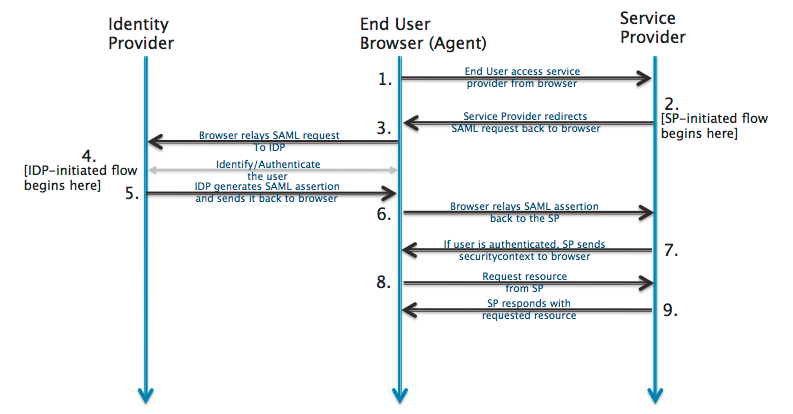
\includegraphics[width=1\textwidth]{immagini/sso_flow.png}
        \caption{\textit{Single Sign-On flow}}
        \textbf{Fonte}:
        \href{https://developer.okta.com/docs/concepts/saml/#federated-identity}{developer.okta.com}
        \label{fig: Single Sign-On flow}
    \end{figure}
Nel dettaglio, la attività che dovevo svolgere per questo progetto erano diverse. Per prima cosa dovevo trovare un protocollo di autenticazione che fosse adeguato alle esigenze dell'azienda e al problema da risolvere. Successivamente, dovevo passare alla progettazione di un sistema di autenticazione di base, che permettesse di effettuare il \textit{login} su \gls{zcsg} tramite \gls{okta}. Dal punto di vista pratico, all'utente era sufficiente cliccare su un'applicazione \gls{okta} presente nel pannello di controllo \gls{okta}, oppure disponibile tramite estensione per \textit{browser}.
\newpage
    \begin{figure}[ht]
        \centering
        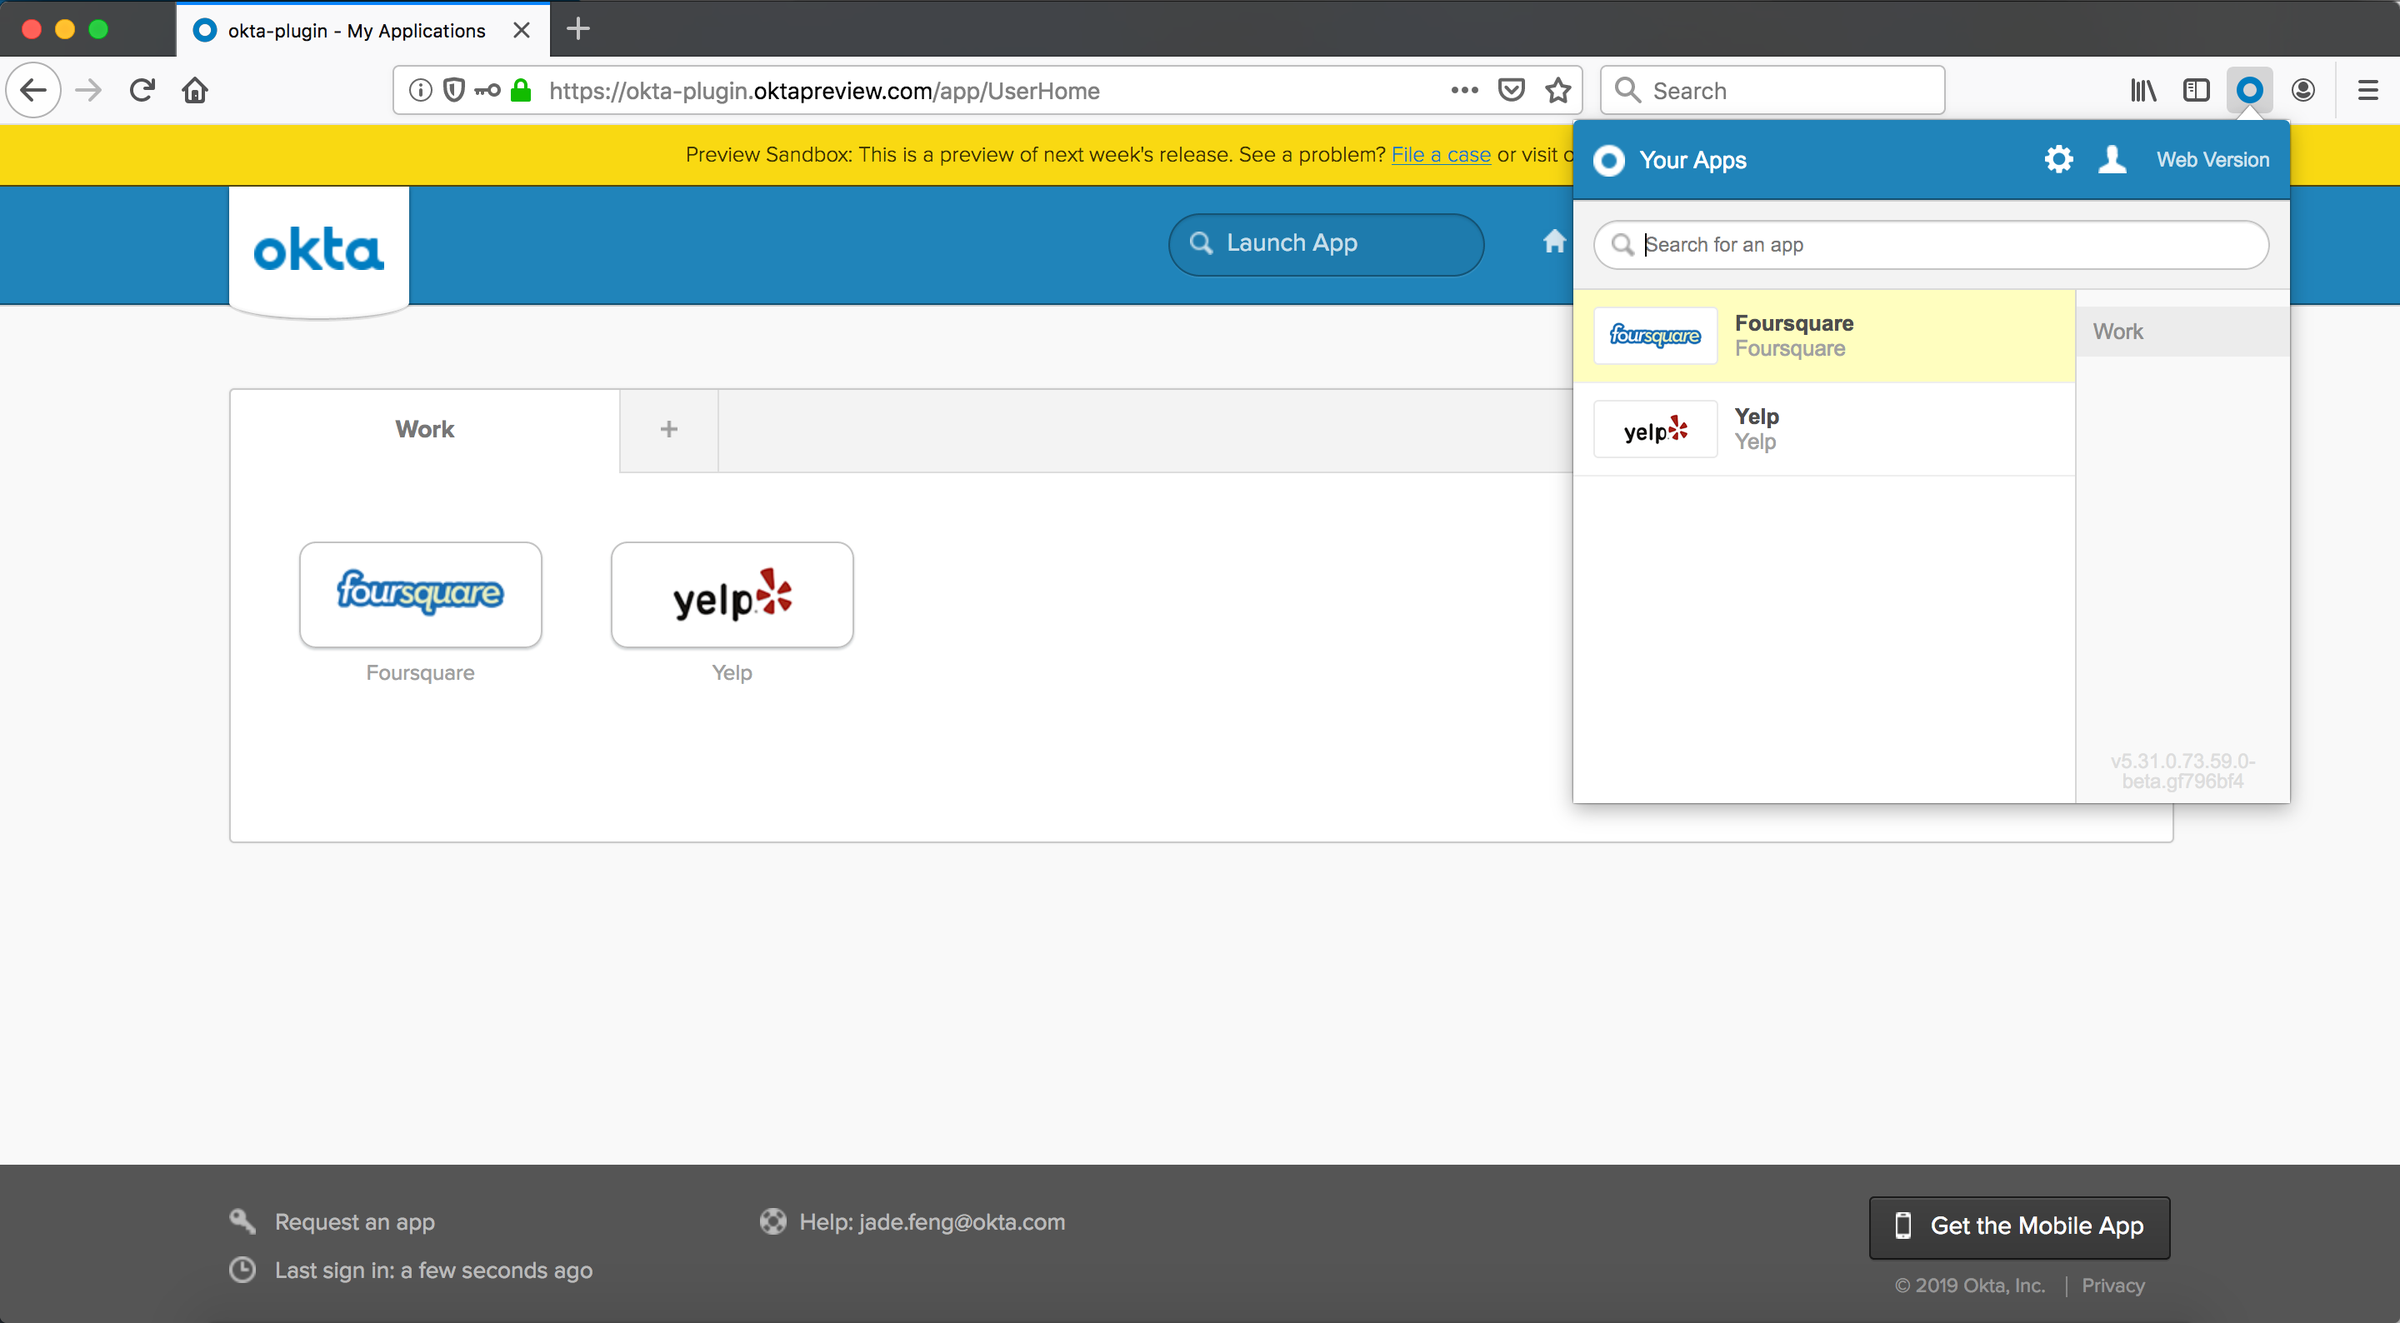
\includegraphics[width=0.9\textwidth]{immagini/okta_plugin.png}
        \caption{\textit{Okta plug-in}}
        \textbf{Fonte}:
        \href{https://addons.mozilla.org/en-US/firefox/addon/okta-browser-plugin/}{addons.mozilla.org}
        \label{fig: Okta plug-in}
    \end{figure}
    
Una volta effettuata l'autenticazione su \gls{okta} e premuto il pulsante relativo al \textit{login} per \gls{zcsg}, l'utente viene reindirizzato sulla \textit{webmail} di \gls{zcsg}.
Oltre a questa funzionalità era richiesto di creare un nuovo \textit{account} su \gls{zcsg} qualóra l'utente \gls{okta} che stesse effettuando un tentativo di accesso ne fosse sprovvisto e, allo stesso tempo, fare una mappatura tra i gruppi ai quali l'utente appartiene su \gls{okta} con le \gls{distlistg} e una \gls{cosg} di \gls{zcsg}. Per fare ciò, dovevo progettare un sistema apposito per stabilire come la mappatura dovesse avvenire, dato che le informazioni tra i due sistemi potevano spesso risultare incompatibili. \\
L'architettura dell'intero sistema doveva essere un'estensione di \textbf{Zextras} che sfruttasse l'utilizzo di un \textit{handler http} ovvero un servizio che riceve delle richieste \textit{\gls{httpg}} nelle stesse modalità di una \textit{\gls{restg}}. Questo \textit{handler} doveva gestire lo scambio di informazioni tra \gls{zcsg} e \gls{okta}, processarle e infine eseguire le operazioni descritte in precedenza.

\section{Pianificazione}
La prima pianificazione delle attività da svolgere è stata fatta da me, insieme al \textit{tutor}, prima dell'inizio dello stage, per poter avere un'idea generale delle tempistiche necessarie al completamento degli obiettivi. Come descritto nella sezione \secref{sec:vincoli_tempo}, la pianificazione originaria ha subito delle leggere modifiche, causa necessità di più tempo da dedicare ad alcune attività. Inoltre, pur seguendo il piano di lavoro originale, la pianificazione di ciò che andava fatto ogni settimana veniva confermato una volta completato il lavoro attualmente in corso.
Infatti dopo gli incontri formali fissati dal \textit{Project Manager} in cui dovevo mostrare i progressi tramite una \textit{\gls{demog}}, vi erano spesso delle nuove richieste oppure delle modifiche da effettuare a ciò che avevo presentato. Per questo motivo, dopo ciascuno di questi incontri, mi fermavo per discutere con il \textit{team} quanto emerso e decidere di conseguenza come agire. \\
Il lavoro da svolgere era suddiviso in due attività principali: l'analisi dei protocolli di autenticazione più diffusi sul mercato, seguita dalla progettazione e implementazione del sistema di autenticazione che utilizzasse il protocollo scelto.
\subsection{Analisi stato dell'arte protocolli di autenticazione}\label{sec:att_analisi}
    La prima attività che ho dovuto svolgere era la ricerca e lo studio dei protocolli di autenticazione più diffusi e utilizzati sul mercato. L'azienda conosceva già alcuni di questi, ma voleva avere un'analisi approfondita e degli esempi del loro utilizzo. Inoltre poteva rivelarsi una valida occasione per scoprire nuovi possibili protocolli adatti all'implementazione del sistema di autenticazione. \\
    L'azienda ha quindi richiesto di redigere un documento che riportasse tutti i risultati delle mie ricerche, in particolare l'analisi dei vantaggi e degli svantaggi di ciascun protocollo e la sua applicabilità al problema da risolvere.
    Durante questo periodo mi sono dedicato allo studio individuale dei protocolli e ho gestito il mio tempo autonomamente. Ogni giorno, durante il \textit{daily scrum} (\secref{sec:met_svilpuppo}), aggiornavo il \textit{team} sui miei progressi e nel resto della giornata mi consultavo con loro in caso di necessità.

    \subsection{Progettazione di un sistema di autenticazione personalizzato} \label{sec:att_progett}
        In seguito all'analisi svolta, il secondo obiettivo dello stage era la progettazione, seguita dall'implementazione, di un sistema di autenticazione per \gls{zcsg} utilizzando il protocollo scelto da me, guidato dal \textit{team} di sviluppo. Il sistema di autenticazione doveva essere in grado di:
        \begin{itemize}
            \setlength\itemsep{0em}
            \item utilizzare \gls{okta} come \textit{\gls{idpg}};
            \item supportare altri \textit{\gls{idpg}} che supportano lo stesso protocollo;
            \item supportare il \textit{login} su \gls{zcsg} tramite il \textit{\gls{ssog}} di \gls{okta} rendendo opzionale l'accesso tramite \textit{email} e \textit{password};
            \item garantire sicurezza.
        \end{itemize}
    \begin{figure}[ht]
        %\setlength{\textfloatsep}{1pt}
        %\setlength{\belowcaptionskip}{1pt}
        \centering
        
\includegraphics[width=0.7\textwidth]{immagini/rd.jpg}
        \caption{\textit{Research \& Development}}
        \textbf{Fonte}:
        \href{https://youteam.io/blog/research-and-development-the-fourth-pillar-of-software-development/}{youteam.io}
        \label{fig: Research & Development}
    \end{figure}

\newpage

La seconda attività, descritta nella sezione \secref{sec:att_progett}, si è rivelata essere quella che ha consumato più tempo di quanto preventivato poiché, anche il \textit{team} non aveva mai fatto uso diretto di questo protocollo e quindi non poteva darmi delle risposte immediate in caso di necessità.\\
Tuttavia, una volta superato questo ostacolo, il lavoro è proseguito secondo il piano di lavoro originale con alcune accelerazioni nell'implementazione di alcuni requisiti che si sono rivelati essere piuttosto semplici. Nella parte finale dello stage ho avuto inoltre la possibilità di eseguire delle attività fuori pianificazione, infatti ho effettuato alcune modifiche al prodotto subito dopo il suo rilascio.


\section{Analisi}\label{sec:requisiti}
Come già discusso nella sezione \secref{sec:att_analisi}, l'attività di ricerca e analisi dei protocolli di autenticazione, è stata la prima ad essere portata a termine. Infatti, nei primi giorni di stage abbiamo discusso con il \textit{team} per stabilirne le modalità. Successivamente abbiamo individuato il primo requisito principale, ovvero l'autenticazione base di un utente su \gls{zcsg} tramite l'\textit{\gls{idpg}} \gls{okta}. Il resto dei requisiti sono stati analizzati nel dettaglio dopo l'implementazione del primo, poiché ci serviva avere una base di partenza funzionante, al fine di capire cosa si potesse implementare e cosa invece non fosse fattibile. \\
Dopo aver capito le possibilità che avevamo, abbiamo stabilito che il sistema da progettare doveva essere modulare dal punto di vista degli \textit{\gls{idpg}} supportati e, allo stesso tempo, dovevamo avere la possibilità di implementare dei servizi specifici per quanto riguarda l'integrazione delle configurazioni utente di \gls{zcsg} e \gls{okta}. Abbiamo dovuto prendere delle decisioni in merito a questo aspetto. Ad esempio l'associazione tra i gruppi ai quali un utente appartiene su \gls{okta} e la \gls{cosg} a cui il corrispettivo utente \gls{zcsg} doveva appartenere poteva essere solo di tipo uno a uno. Per soddisfare un requisito di questo genere ho dovuto pensare ad una soluzione \textit{ad hoc} che richiedeva di fare delle sperimentazioni con un sistema di base funzionante, capace di mettere in atto una comunicazione tra \gls{zcsg} e \gls{okta}. \\
I requisiti raccolti in seguito all'attività di analisi sono:
\begin{itemize}
    \setlength\itemsep{0em}
    \item \textbf{Obbligatori}: 14;
    \item \textbf{Desiderabili}: 1;
    \item \textbf{Opzionali}: 2;
\end{itemize}
 
Alcuni di questi sono illustrati nella seguente tabella:

\newpage

\begin{center}
    \begin{table}[h]
    \def\arraystretch{2}
    \begin{tabular}{| p{3cm} | p{9cm} |} % you can change the dimension according to the spacing requirements 
        \hline
        \textbf{Identificativo} & \textbf{Descrizione} \\ \hline  
        R01 & Autenticare un utente non esistente su \gls{zcsg} tramite \gls{okta}, previa creazione dell'\textit{account}\\ \hline
        R05 & Durante il processo di creazione di un nuovo utente su \gls{zcsg}, aggiungerlo alle giuste \gls{distlistg} a seconda dei gruppi ai quali appartiene su \gls{okta}\\ \hline
        R08 & Durante la fase di autenticazione su \gls{zcsg} effettuata tramite \gls{okta}, aggiornare le \gls{distlistg}, se i gruppi ai quali cui l'utente appartiene su \gls{okta} sono cambiati\\ \hline
        R11 & Configurazione del protocollo \textit{\gls{saml}} a livello di dominio\\ \hline
        R14 & Autenticazione a due fattori\\ \hline 
    \end{tabular}
    \caption{Tabella parziale dei requisiti}
    \end{table}
\end{center}

%**************************************************************
\section{Scelta del protocollo di autenticazione}
In seguito all'analisi condotta sui protocolli di autenticazione, già accennata nella sezione \secref{sec:att_analisi}, sono emersi due protocolli di interesse, che ho proposto e discusso insieme al \textit{team}.
I due protocolli individuati erano \textit{\gls{samlg}} e \gls{openidg}. Di seguito illustrerò i vantaggi e gli svantaggi di ciascuno.

\subsection{SAML (Security Assertion Markup Language)}
    \subsubsection{Vantaggi}
    \begin{itemize}
        \item fornisce meccanismi di sicurezza nel momento in cui la connessione \textit{HTTPS} non è disponibile o potrebbe essere compromessa;
        \item si tratta di uno dei protocolli più utilizzati e affermati sul mercato;
        \item se implementato correttamente è molto affidabile e sicuro;
        \item il meccanismo chiamato \textit{federated identity} permette di ridurre i costi per la gestione delle identità degli utenti che hanno accesso a servizi di più organizzazioni.
    \end{itemize}
    \subsubsection{Svantaggi}\label{sec:saml_svantaggi}
    \begin{itemize}
        \item nell'implementazione di alcuni casi d'uso è necessario effettuare dei reindirizzamenti \textit{\gls{httpg}}, che conviene eseguire con una richiesta \textit{POST}. Il problema risiede nel fatto che per poterla fare in automatico è necessario scrivere del codice aggiuntivo con un altro linguaggio;
        \item per il problema evidenziato al punto precedente, non è facile implementare questo protocollo su applicazioni native per dispositivi mobili;
        \item essendo un protocollo basato su \textit{\gls{xmlg}}, soffre di una tipologia di attacchi chiamati \textit{XML Signature Wrapping}, che potrebbero modificare i documenti \textit{\gls{xmlg}} scambiati tra gli interlocutori del protocollo;
        \item l'\textit{\gls{xmlschemag}} del protocollo è particolarmente complesso.
    \end{itemize}

\subsection{OpenID}
    \subsubsection{Vantaggi}
    \begin{itemize}
        \setlength\itemsep{0em}
        \item i \textit{\gls{jsong} Web Token (JWT)} utilizzati per rappresentare le informazioni dell'autenticazione sono in un formato portabile e moderno e supportano diversi algoritmi di crittografia;
        \item essendo basato su un altro protocollo chiamato \gls{oauthg}, il quale funziona su applicazioni native per dispositivi mobili, permette di essere implementato facilmente su di esse;
        \item essendo basato su un protocollo di autorizzazione, citato al punto precedente, con \gls{openidg} si ha un singolo protocollo per autenticazione e autorizzazione;
        \item Facile da implementare.
    \end{itemize}
    \subsubsection{Svantaggi}
    \begin{itemize}
        \setlength\itemsep{0em}
        \item al momento dell'analisi effettuata risultava essere una soluzione poco comune sul mercato, da ciò ne deriva la mancanza di \textit{best practice};
        \item \textit{HTTPS} è l'unico livello di criptazione e sicurezza tra il \textit{client} e l'\textit{\gls{idpg}}.
    \end{itemize}

\subsection{Motivazioni della scelta}
Dopo una discussione con il \textit{team} di sviluppo e il \textit{Project Manager}, abbiamo preso la decisione di utilizzare il protocollo \textit{\gls{samlg}}. Le ragioni che ci hanno portato a sceglierlo sono le seguenti:
\begin{itemize}
    \item essendo il protocollo molto diffuso, vi erano \textit{best practice} note e una comunità di sviluppatori su cui fare affidamento;
    \item \gls{okta} supporta questo protocollo facilitando la comunicazione con un servizio personalizzato che implementa \gls{samlg};
    \item disponibilità di una \gls{libg} scritta in \textit{Java}, il linguaggio utilizzato in azienda, già affermata e utilizzata in altre applicazioni, che implementa le funzionalità base del protocollo. Tale libreria è \textit{\gls{opensg}}, di fondamentale importanza data la filosofia aziendale;
    \item non vi era necessità di portare questo sistema di autenticazione su dispositivi mobili ma, nel caso in futuro ci fosse la necessità di farlo, ci sarebbero delle soluzioni valide per risolvere il problema descritto nella sezione \secref{sec:saml_svantaggi}.
\end{itemize}

\subsection{Il protocollo SAML}
\subsubsection{Attori SAML}
Il protocollo \textit{\gls{samlg}} coinvolge generalmente tre attori:
\begin{itemize}
    \item \textit{\textbf{Service provider}}: è l'entità che fornisce il servizio all'utente, solitamente un sito \textit{web} o una risorsa disponibile su di esso. In questo progetto è la \textit{webmail} di \gls{zcsg};
    \item \textit{\textbf{User-agent}}: è un software permette la fruizione dei contenuti ad un utente. Di solito un \textit{web browser} che renderizza i contenuti delle pagine \textit{web};
    \item \textit{\textbf{Identity Provider}}: è l'autorità che certifica l'identità di un utente. In questo progetto questo ruolo è assunto da \gls{okta}.
\end{itemize}
Un esempio di come queste tre parti interagiscono è illustrato nella figura \secref{fig: Single Sign-On flow}.
\subsubsection{Componenti SAML}
\textit{\gls{samlg}} è costituito da diversi componenti che possono essere combinati tra di loro in diversi modi, a seconda del caso d'uso richiesto dal problema da risolvere. Le principali funzioni di questi componenti sono autenticazione, gestione dell'identità e autorizzazione tra organizzazioni che abbiano stabilito un rapporto di fiducia. I principali "concetti" del protocollo sono i seguenti:
\begin{itemize}
    \item \textit{\textbf{Assertion}}: è un documento in formato \textit{\gls{xmlg}} che contiene le informazioni sull'autenticazione e/o autorizzazione di un utente. Tale documento è solitamente generato dall'\textit{\gls{idpg}} e inviato al \textit{\gls{spg}};
    \item \textit{\textbf{Protocols}}: sono dei meccanismi per fare in modo che le richieste e le risposte \textit{\gls{samlg}} siano compatibili tra loro;
    \item \textit{\textbf{Bindings}}: definiscono il metodo di comunicazione a basso livello utilizzato dai partecipanti del protocollo. Per esempio permettono di specificare se la comunicazione avviene tramite richieste \textit{\gls{httpg}} o \textit{\gls{soapg}};
    \item \textit{\textbf{Profiles}}: i profili definiscono una particolare configurazione di \textit{assertion}, \textit{protocols} e \textit{bindings} che serve per soddisfare un caso d'uso specifico;
    \item \textit{\textbf{Metadata}}: è un documento \textit{\gls{xmlg}} che serve per condividere delle configurazioni tra due parti. Per esempio il metodo di crittografia delle \textit{\gls{samlass}} o di un insieme di attributi;
    \item \textit{\textbf{Authentication Context}}: è un meccanismo, definito da un \textit{\gls{xmlschemag}}, che serve per descrivere la tipologia di autenticazione impiegata dall'utente quando si autentica con l'\textit{\gls{idpg}}.
\end{itemize}

\newpage

    \begin{figure}[ht]
        \centering
        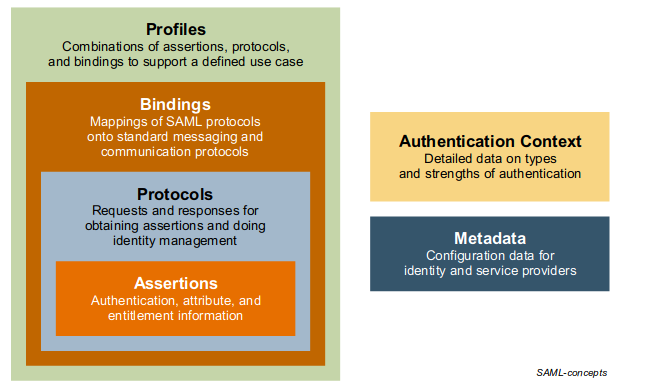
\includegraphics[width=0.8\textwidth]{immagini/SAMLCore.png}
        \caption{\textit{SAML Core concepts}}
        \textbf{Fonte}:
        \href{https://www.oasis-open.org/committees/download.php/27819/sstc-saml-tech-overview-2.0-cd-02.pdf}{oasis-open.org}
        \label{fig: SAML core}
    \end{figure}

\section{Progettazione}
\subsection{Configurazione applicazione Okta}
Un'applicazione \gls{okta} è un servizio basato sullo scambio di informazioni tramite \textit{\gls{restg}} tra \gls{okta} e un altro servizio \textit{web}. Sapendo che \gls{okta} supportava il protocollo \textit{\gls{samlg}} e che in azienda erano state già create altre applicazioni \gls{okta} per integrazioni con gli strumenti utilizzati internamente, abbiamo stabilito che la cosa migliore da fare per comunicare con l'\textit{\gls{idpg}} fosse quella di creare una \textit{\gls{samlg}} \textit{application} che avesse come \textit{\gls{endpointg}} l'indirizzo dell'\textit{handler} \textit{\gls{httpg}} descritto nella sezione successiva.
Di seguito un esempio di configurazione della \textit{\gls{samlg}} \textit{application} di \gls{okta} con gli \textit{\gls{endpointg}} dell'\textit{handler} \textit{\gls{httpg}}.

    \begin{figure}[ht]
        \centering
        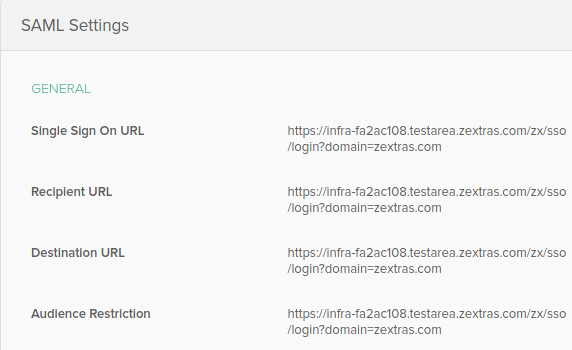
\includegraphics[width=0.8\textwidth]{immagini/endpoints.png}
        \caption{\textit{SAML endpoints}}
        \label{fig: SAML endpoints}
    \end{figure}
    
Essendo questa un'applicazione specifica per \textit{\gls{samlg}}, era possibile specificare quali attributi dell'utente inviare all'\textit{handler} \textit{\gls{httpg}} (per esempio l'anagrafica e i gruppi ai quali appartiene su \gls{okta}) per avere la possibilità non solo di autenticarlo, ma anche di creare il nuovo \textit{account} su \gls{zcsg} come già speficificato nella sezione \secref{sec:progetto}. Tali informazioni vengono inviate all'\textit{handler} \textit{\gls{httpg}} tramite una \textit{\gls{samlass}}. Di seguito un esempio di configurazione:

    \begin{figure}[ht]
        \centering
        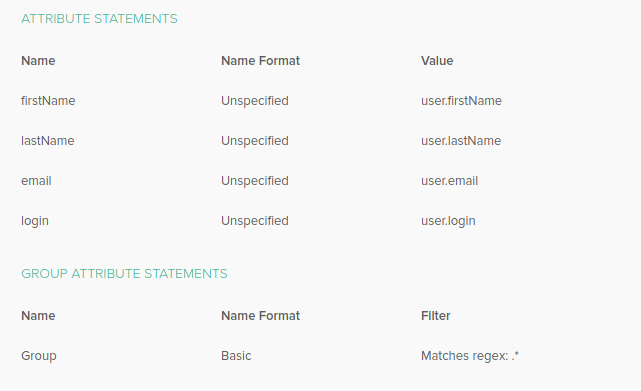
\includegraphics[width=0.8\textwidth]{immagini/saml_attributes.png}
        \caption{Attributi \textit{SAML}}
        \label{fig: Attributi SAML}
    \end{figure}

\subsection{Progettazione handler HTTP}
I servizi \textit{web} di \textbf{Zextras} sono gestiti tramite degli \textit{handler} \textit{\gls{httpg}}, ovvero delle classi \textit{Java} che restano in ascolto su uno o più \textit{\gls{endpointg}} tramite i quali ricevono dei dati. Questi vengono elaborati e viene generata una risposta che può ridursi ad un'azione eseguita, un messaggio di ritorno oppure un reindirizzamento ad una certa pagina \textit{web}. In particolare l'\textit{handler} \textit{\gls{httpg}} che gestiva tutte le operazioni che il mio sistema doveva svolgere, doveva ricevere una \textit{SAML Response}, cioè un documento \textit{\gls{xmlg}} con una \textit{\gls{samlass}} al suo interno. L'asserzione conteneva i dati dell'utente con i quali era possibile:
\begin{itemize}
    \setlength\itemsep{0em}
    \item autenticare l'utente;
    \item creare il nuovo \textit{account} su \gls{zcsg} al primo tentativo di \textit{login};
    \item assegnare l'utente alla giusta \gls{cosg} e alle \gls{distlistg}.
\end{itemize}
\subsection{Sistema di mappatura dei gruppi Okta}
Una volta giunti i dati all'\textit{handler} \textit{\gls{httpg}} era necessario prendere una decisione su come mappare i gruppi ai quali l'utente apparteva su \gls{okta} con una sola \gls{cosg} e allo stesso tempo più \gls{distlistg} di \gls{zcsg}. Purtroppo non era possibile eseguire questa operazione in automatico poiché se un utente apparteneva ad un gruppo chiamato \texttt{A} su \gls{okta}, il sistema avrebbe dovuto inserire l'utente in una \gls{cosg} chiamata \texttt{A}. Ma non era scontata la presenza di una \gls{cosg} di nome \texttt{A} su \gls{zcsg}. Il problema è analogo per le \gls{distlistg}, in quanto un gruppo di nome \texttt{A} doveva essere mappato sulla lista denominata \texttt{A@dominio}, ma l'esistenza di tale dominio su \gls{zcsg} non era garantita. Per i motivi sopra elencati, tentare una mappatura automatica avrebbe portato ad errori e comportamenti inattesi. \\
Ho investito un po' di tempo per cercare una soluzione e ho proposto di dare la possibilità all'amministratore di \gls{okta} e \gls{zcsg} di configurare manualmente le associazioni desiderate tramite un \textit{file} in formato \textit{\gls{jsong}}. Nel caso della \gls{cosg}, la quale è unica per ciascun utente, era possibile effettuare un'associazione uno a uno tra gruppo di \gls{okta} e \gls{cosg}, a patto che questa esistesse su \gls{zcsg}. In caso contrario il sistema avrebbe ignorato l'associazione in fase di mappatura. Per quanto riguarda le \gls{distlistg}, era possibile associare un gruppo \gls{okta} con più di \gls{distlistg} presenti su \gls{zcsg}.
Una volta discussa e approvata dal \textit{team} e dal \textit{Project Manager} ho implementato questa soluzione. Di seguito un esempio di mappatura per la \gls{cosg} e le \gls{distlistg}.

    \begin{figure}[ht]
        \centering
        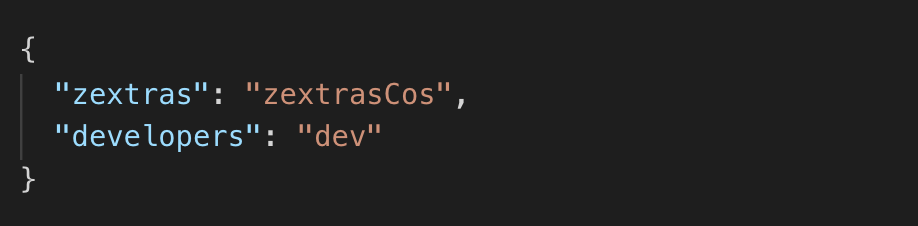
\includegraphics[width=1\textwidth]{immagini/cosMapping.png}
        \caption{Mappatura classe di servizio}
        \label{fig: Mappatura classe di servizio}
    \end{figure}
    
     \begin{figure}[ht]
        \centering
        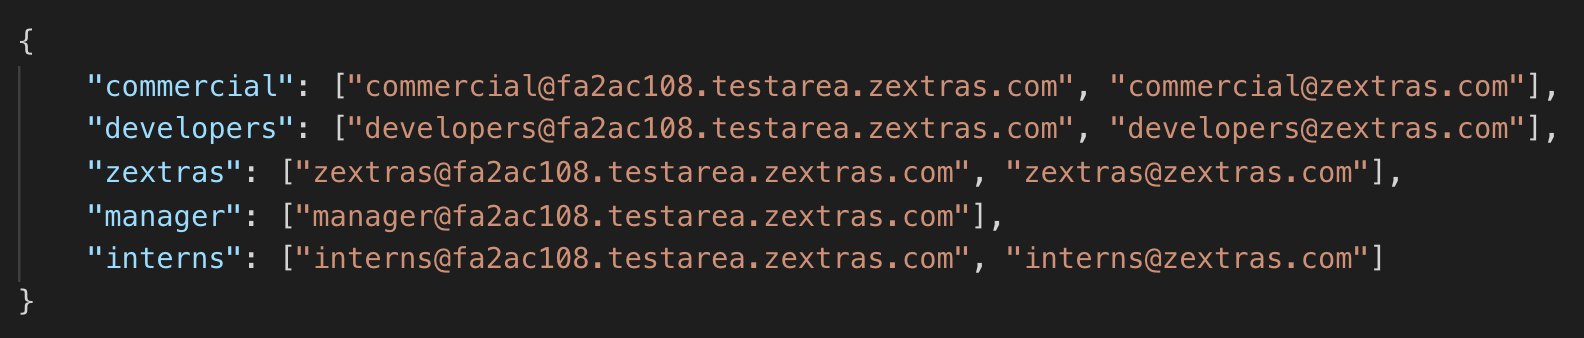
\includegraphics[width=1\textwidth]{immagini/distListMapping.png}
        \caption{Mappatura liste di distribuzione}
        \label{fig: Mappatura liste di distribuzione}
    \end{figure}

\subsection{Configurazione Zimbra}
La configurazione di tutto il sistema di autenticazione l'ho realizzata attraverso la configurazione di \gls{zcsg}, la quale offre la possibilità di definire attributi di diversi tipi, tra cui valori binari (vero o falso), stringhe e oggetti \textit{\gls{jsong}}. Le mappature descritte nella sezione precedente e illustrate nelle figure \secref{fig: Mappatura classe di servizio} e \secref{fig: Mappatura liste di distribuzione} erano configurate attraverso due attributi specifici. Oltre a questi ne ho definiti altri, tra cui:
\begin{itemize}
    \item configurazione del protocollo \textit{\gls{samlg}} (informazioni riguardanti \textit{\gls{idpg}} e \textit{\gls{spg}});
    \item cttivazione e disattivazione della creazione automatica di un nuovo \textit{account}  su \gls{zcsg};
    \item cttivazione e disattivazione della sincronizzazione dei gruppi \gls{okta} ai quali appartiene un utente, con \gls{cosg} e \gls{distlistg} ad ogni accesso tramite \textit{\gls{samlg}}.
\end{itemize}
Questi attributi vengono letti dall'\textit{handler} \textit{\gls{httpg}} ogni volta che il sistema di autenticazione riceve una richiesta.

\section{Sviluppo}
In questa sezione illustrerò alcuni dettagli riguardanti l'implementazione, in particolare alcuni ostacoli che ho dovuto superare per proseguire con lo sviluppo.
\subsection{Libreria SAML} \label{sec:libreria}
Per poter estrapolare i dati in arrivo dalla \textit{SAML Response} di \gls{okta} era necessario avere un modo per poter effettuare il \textit{\gls{parsingg}} del documento \textit{\gls{xmlg}}. Tuttavia non c'era tempo a sufficienza per poter progettare e implementare da zero, un \textit{parser} in grado di gestire i documenti \textit{\gls{xmlg}} generati da \textit{\gls{samlg}}, poiché questi hanno una struttura molto complessa.

    \begin{figure}[ht]
        \centering
        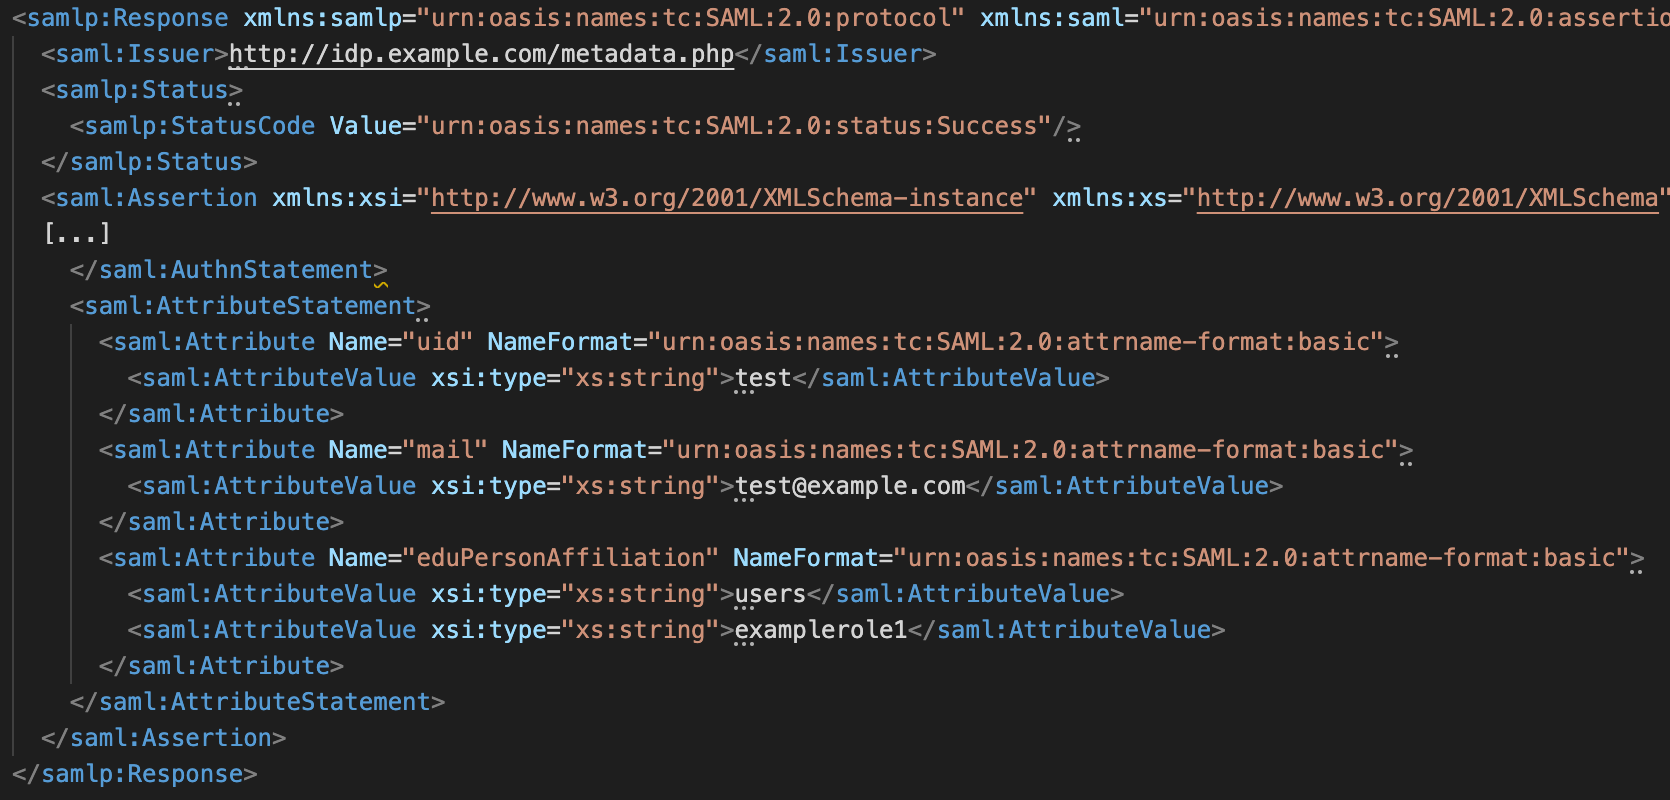
\includegraphics[width=1\textwidth]{immagini/saml_response.png}
        \caption{\textit{SAML Response}}
        \textbf{Fonte}:
        \href{https://www.samltool.com/generic_sso_res.php}{samltool.com}
        \label{fig: SAML Response}
    \end{figure}
    
Per fare ciò ho incluso una \gls{libg} \textit{\gls{opensg}} che, data una \textit{SAML Response}, restituiva una \gls{struttdatig} contenente i dati necessari, estrapolati dai \textit{tag} \texttt{<saml:AttributeValue>} come illustrato in figura \secref{fig: SAML Response}.

\newpage

Tuttavia, l'introduzione di questa libreria ha portato alla luce nuove problematiche. Questa, utilizzava la gestione delle richieste e risposte \textit{\gls{httpg}} tramite le classi della \textit{\gls{apig}} di \textit{Java}, in particolare utilizzava il \textit{package} \texttt{javax.servlet.http} \footnote{\url{https://javaee.github.io/javaee-spec/javadocs/javax/servlet/http/package-summary.html}}. \textbf{Zextras}, invece, utilizzava un \textit{\gls{frameworkg}} chiamato \textit{Netty} \footnote{\url{https://netty.io/}}, pertanto c'era una situazione di incompatibilità. Ho quindi dovuto provvedere ad adattare tutti i metodi della \gls{libg} affinché fossero compatibili con il \textit{\gls{frameworkg}} utilizzato dall'azienda. \\

\section{Documentazione}
La documentazione ha fatto parte dei miei compiti sin dall'inizio dell'attività di stage, rivelandosi materiale utile per diversi motivi. Per tutto il \textit{team}, soprattutto per coloro che non hanno lavorato direttamente con me, ma che necessitano di sapere come funzionano alcuni aspetti del prodotto (per esempio i sistemisti devono sapere come effettuare le configurazioni sul \textit{server}). Inoltre è di fondamentale importanza per chi ora dovrà effettuare la manutenzione, dato che potrà risalire facilmente a tutto il lavoro da me svolto. Infine mi è stata molto di aiuto durante la presentazione dei miei progressi durante gli incontri con il \textit{Project Manager}.

\subsection{Documenti tecnici e manuali}
Durante l'attività descritta nella sezione \secref{sec:att_analisi}, ho documentato tutti i risultati dei miei studi in un documento che illustrava tutti i protocolli analizzati, riportando le informazioni tecniche essenziali e discutendone vantaggi e svantaggi per ciascuno di essi. Questo documento è stato poi aggiornato fino al momento in cui, insieme al \textit{team}, abbiamo scelto il protocollo da utilizzare. \\
Per quanto riguarda la documentazione del prodotto sviluppato, ho scritto un manuale contenente informazioni circa la progettazione del sistema di autenticazione e i passi per poterlo configurare correttamente. Il documento, accessibile a tutti i reparti dell'azienda, era necessario ai sistemisti per poter installare e opportunamente configurare il sistema e al \textit{team}, nel caso in futuro dovesse estenderlo o apportare delle correzioni.
Lo strumento utilizzato per la gestione di questi documenti è \textbf{Confluence}, come descritto nella sezione \secref{sec:doc}.

\subsection{Codice sorgente}
La documentazione del codice è fondamentale per due motivi: spiegare sezioni di codice difficili da comprendere e facilitare la manutenzione a coloro che dovranno farla, soprattutto se verrà fatta da persone diverse dall'autore. Infatti in una \textit{Sprint Retrospective}, in particolare durante la scrittura dello \textit{Starfish Retrospective} (come descritto nella sezione \secref{sec:met_svilpuppo}) è emerso che tutto il \textit{team} avrebbe dovuto dedicare più tempo alla documentazione del codice, scrivendola secondo le regole del \gls{javadocg}.


\section{Verifica e Validazione}
\subsection{Verifica}
Come descritto nella sezione \secref{sec:verifica}, in azienda abbiamo attuato diverse tecniche e strumenti per verificare che i prodotti sviluppati non contenessero errori. La verifica automatica avviene tramite \textbf{Jenkins}, il quale ha una \textit{pipeline} configurata in modo da mettere in funzione il ciclo di \textit{\gls{cig}} e \textit{\gls{cdg}} ad ogni \textit{commit} sul \textit{\gls{repositoryg}}, illustrato nella figura \secref{fig: Continuous Integration}.
\subsubsection{Test}
All'interno della \textit{pipeline} della \textit{\gls{cig}} vi era l'esecuzione automatica delle varie tipologie di \textit{test} (per esempio \textit{test} di unità e \textit{test} di integrazione). Poiché il progetto da me sviluppato interagiva con molte parti dell'architettura di \textbf{Zextras}, ho scritto solo \textit{test} di integrazione. I \textit{test} sono parte fondamentale dello sviluppo \textit{software} e meritano di essere progettati e mantenuti allo stesso modo del codice di produzione. Per fare ciò, ho utilizzato due strumenti:
\begin{itemize}
    \item \textbf{Mockito}: è un \textit{\gls{frameworkg}} che facilita la scrittura dei \textit{test} in \textit{Java}; 
    \item \textbf{Guice}: è un \textit{\gls{frameworkg}} \textit{\gls{opensg}} per il linguaggio \textit{Java}, sviluppato da \textbf{Google}, che permette di applicare in modo semplice e scalabile la \textit{\gls{depinjg}}.
\end{itemize}
Di seguito una tabella con alcuni di essi:

\begin{center}
    \begin{table}[h]
    \def\arraystretch{1.65}
    \begin{tabular}{|p{3cm}|p{7cm}|p{2cm}|}
        \hline
        \textbf{Identificativo} & \textbf{Descrizione} & \textbf{Esito} \\ \hline  
        IT01 & Se un utente è inserito in più gruppi \gls{okta} mappati con la corrispondente \gls{cosg}, allora il sistema non assegna nessun \gls{cosg} all'utente & \textcolor{ForestGreen}{Superato}\\ \hline
        IT04 & Se la creazione automatica dell'\textit{account} è disabilitata viene mostrata una pagina di errore informativa per l'utente & \textcolor{ForestGreen}{Superato}\\ \hline
        IT05 & Quando un utente effettua il \textit{login}, vengono aggiornate le \gls{distlistg} alle quali appartiene se i suoi gruppi di \gls{okta} sono cambiati & \textcolor{ForestGreen}{Superato}\\ \hline
        IT07 & Se un utente tenta di autenticarsi da \gls{okta} per la prima volta, gli viene creato un nuovo \textit{account} su \gls{zcsg}, associato al profilo \gls{okta} & \textcolor{ForestGreen}{Superato}\\ \hline
        IT10 & Se l'utente tenta di accedere a \gls{zcsg} senza essere autenticato su \gls{okta}, viene reindirizzato sulla pagina di \textit{login} di \gls{okta} & \textcolor{ForestGreen}{Superato}\\ \hline
    \end{tabular}
    \caption{Tabella parziale dei \textit{test} di integrazione}
    \end{table}
\end{center}

I \textit{test} da me progettati e implementati erano in numero sufficiente secondo il parere del \textit{team}, tuttavia l'introduzione della \gls{libg} descritta nella sezione \secref{sec:libreria} mi ha portato ad avere una copertura del codice piuttosto bassa, circa del 40\%. Questo perché il codice presente nella \gls{libg} offriva molteplici funzionalità che non ho avuto bisogno di utilizzare. Ai fini qualitativi è comunque accettabile perché per motivi di tempo non c'è stata la possibilità di testare a fondo il modulo \textit{software} introdotto.

\subsubsection{Code review}
Le \textit{\gls{codereviewg}} rappresentano un altro strumento di verifica, in questo caso non automatica. Ad ogni nuova \textit{pull request} sul \textit{\gls{repositoryg}} vengono assegnati dei revisori, con il compito di analizzare il codice scritto da un altro membro del \textit{team}. Se il codice rispetta gli standard di qualità, la \textit{pull request} viene approvata con conseguente \textit{merge} sul \textit{branch} principale del \textit{\gls{repositoryg}}, altrimenti l'autore del codice deve risolvere quanto segnalato dai revisori prima di poter sottoporre il codice ad una nuova revisione. Le \textit{\gls{codereviewg}} sono molto utili sia per assicurare che il codice scritto sia conforme alle norme di codifica, sia per confrontare la soluzione implementata con il resto del \textit{team}.

    \begin{figure}[ht]
        \centering
        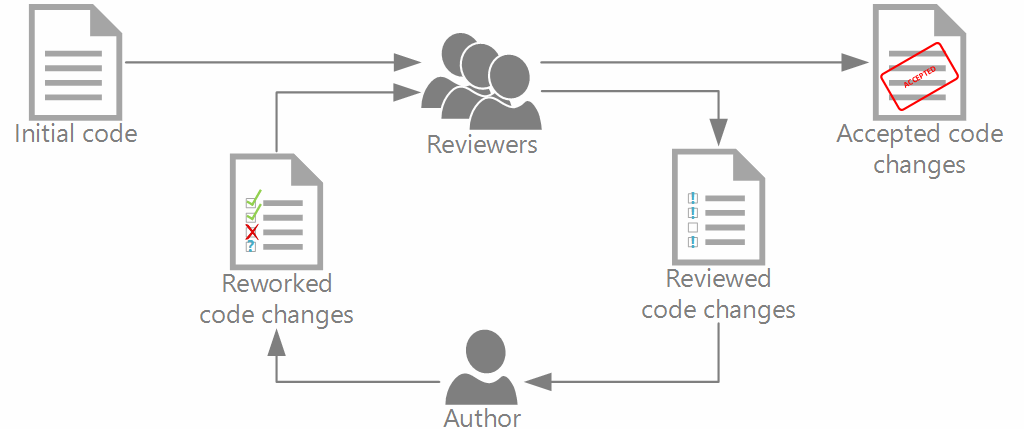
\includegraphics[width=1\textwidth]{immagini/code_review.png}
        \caption{\textit{Code review flow}}
        \textbf{Fonte}:
        \href{https://storage.googleapis.com/causecode-wordpress-media/2019/01/97795825-code-review-process-1024x429.png}{causecode.com}
        \label{fig: Code review flow}
    \end{figure}

\subsection{Validazione}
Gli incontri formali con il \textit{Project Manager} e alcuni membri del \textit{team} di sviluppo sono serviti fin da subito per controllare lo stato di avanzamento dello sviluppo del prodotto. Infatti già alla dimostrazione della prima \textit{\gls{demog}} avevo implementato le funzionalità di base del sistema di autenticazione e ricevuto i primi \textit{feedback}. Da ciò ne conseguiva il tracciamento dei requisiti soddisfatti e di quelli ancora da soddisfare.
L'ultimo incontro si è tenuto il giorno 6/12/2019 a cui hanno partecipato:
    \begin{itemize}
            \item il \textit{CEO} dell'azienda;
            \item il \textit{Project Manager};
            \item il responsabile tecnico dell'azienda;
            \item il \textit{team} di sviluppo con il \textit{tutor} aziendale;
            \item il responsabile di un altro \textit{team};
    \end{itemize}
Durante questa riunione ho mostrato il sistema di autenticazione in azione e abbiamo attestato il soddisfacimento dei requisiti stabiliti durante l'attività di analisi, descritta nella sezione \secref{sec:requisiti}. Su un totale di 17 requisiti, ne ho implementati 16, circa il 94\%, considerando che uno degli obiettivi inizialmente prefissati è stato in seguito rimosso.
Inoltre abbiamo discusso circa alcuni miglioramenti da apportare all'applicazione. In questa sede il responsabile tecnico ha fatto delle nuove richieste, soprattutto per quanto riguarda la configurazione, al fine di facilitare il lavoro dei sistemisti. Dopo aver messo a punto le ultime sistemazioni e aver accertato che il prodotto fosse conforme alle aspettative iniziali e quelle emerse in seguito, il giorno 11/12/2019, abbiamo rilasciato il prodotto in produzione per l'utilizzo aziendale. \\